Based on six evaluation points the prediction is ..., as illustrated in ref{}, and the probabilities that $\Y(\theta) < 0.30$ are ... .

By comparing figure \ref{} and \ref{}, one .... 

We will suggest the scientist's to use $\theta = ... $. 

\begin{figure}
    \centering
    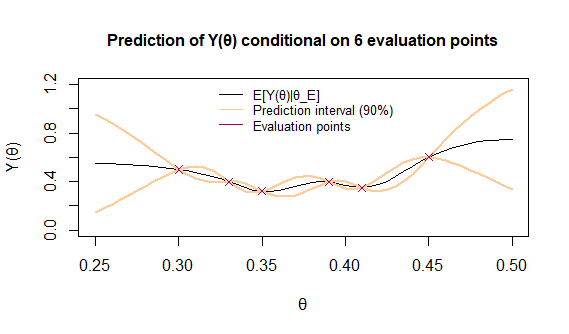
\includegraphics[width=100mm]{2cPred.png}
    \caption{ FIGURTEKST }
    \label{2cPred}
\end{figure}
\begin{figure}
    \centering
    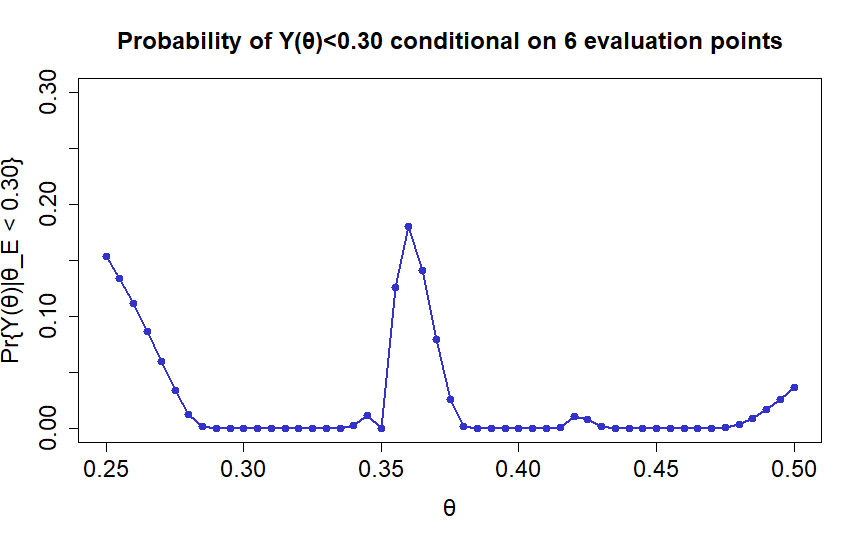
\includegraphics[width=100mm]{2ctheta.png}
    \caption{Prediction of $Y(\theta)$ conditional on the six evaluation points given. The graph includes a $90\%$ prediction interval. }
    \label{2bTheta}
\end{figure}